\documentclass[titlepage,11pt]{article}
\usepackage{comment}
\usepackage{enumitem}
\usepackage{transparent} % Untuk transparansi gambar
\usepackage{listings}
\usepackage{amsmath}
\usepackage{graphicx}
\usepackage[font=small,labelfont=bf]{caption}
\usepackage[bahasa]{babel}
\usepackage{float}
\usepackage{verbatim}
\usepackage{graphicx,tabularx,multirow}
\usepackage{xcolor}
\usepackage[onehalfspacing]{setspace}
\usepackage[
	allcolors=visigrey,
	colorlinks=true,
]{hyperref}
\usepackage[a4paper,left=2cm,right=2cm]{geometry}
% Pengaturan kutipan artikel
\usepackage[style=ieee, backend=biber]{biblatex}
%Code listing style pak akok
\definecolor{codegreen}{rgb}{0,0.6,0}
\definecolor{codegray}{rgb}{0.5,0.5,0.5}
\definecolor{codepurple}{rgb}{0.58,0,0.82}
\definecolor{backcolour}{rgb}{0.95,0.95,0.92}

\usepackage{eso-pic} % Untuk menambahkan elemen ke seluruh halaman

\newcommand\BackgroundPic{
  \put(0,0){
    \parbox[b][\paperheight]{\paperwidth}{
      \vfill
      \centering
      \transparent{0.1}
      \includegraphics[width=0.4\paperwidth,keepaspectratio]{miot.png}
      \vfill
    }
  }
}

\newcommand\BackgroundAllPages{ \AddToShipoutPicture*{\BackgroundPic} }
\newcommand\BackgroundNone{ \ClearShipoutPicture } % hilangkan background

\lstdefinestyle{mystyle}{
	backgroundcolor=\color{backcolour}, commentstyle=\color{codegreen},
	keywordstyle=\color{magenta},
	numberstyle=\small\color{codegray},
	stringstyle=\color{codepurple},
	basicstyle=\ttfamily\footnotesize,
	breakatwhitespace=false,         
	breaklines=true,                 
	captionpos=t,                    
	keepspaces=true,                 
	numbers=left,                    
	numbersep=5pt,                  
	showspaces=false,                
	showstringspaces=false,
	showtabs=false,           
	frame = single,
	tabsize=2
}
\lstset{style=mystyle}

\definecolor{visigrey}{rgb}{.1,.15,.15}
\geometry{top=1cm,bottom=.5cm}
\savegeometry{titlepage}
\geometry{top=2cm,bottom=2cm}
\savegeometry{main}

\def\bspace{\(\qquad\qquad\qquad\)}
\usepackage[T1]{fontenc}
\usepackage[utf8]{inputenc}
\usepackage{tgheros}
\renewcommand*\familydefault{\sfdefault}

\setcounter{tocdepth}{6}

\def\autor{Laboratorium }
\def\lab{Multimedia dan Internet of Things}
\def\departemen{Departemen Teknik Komputer}
\def\institut{Institut Teknologi Sepuluh Nopember}
\def\praktikum{Laporan Sementara \\ Praktikum Jaringan Komputer}
\def\nama{Muhammad Zidane Faiq Sidqi - 5024231040}
% Ubah Judul sesuai dengan modul
\def\judul{Routing dan Manajemen IPv6}
\def\tanggal{2025}
\begin{document}
% Ubah Bahasa sesuai dengan keinginan
\selectlanguage{bahasa}

\BackgroundNone
\def\headingtype{\bf \small}
\loadgeometry{titlepage}

\begin{titlepage}
	\centering
	\begin{tabularx}{\textwidth}{l@{\hskip 0pt}lX}
		\raisebox{-0.5\height}{
\includegraphics[width=3cm]{Cover/img/logodepart.png}} 
		& \raisebox{-0.5\height}{\includegraphics[width=3cm]{Cover/img/miot.png}} 
		& \raggedleft
	\hfill
	\begin{minipage}{0.5\textwidth}
		\raggedleft
		{\emph{\headingtype \autor}} \\[-2pt]
		{\headingtype \lab} \\[-2pt]
		{\headingtype \departemen} \\[-2pt]
		{\headingtype \emph{\institut}}
	\end{minipage}

	\vspace{5cm}
	\end{tabularx}
	
	\vspace{5cm}
	{\Huge \bf \praktikum \par}
	
	\vspace{2cm}
	{\LARGE \bf \judul \par}
	
	\vspace{2cm}
	{\Large \nama \par}
	
	\vfill
	{\Large \tanggal \par}
	
	\vfill
	
\includegraphics[width=\textwidth]{Cover/img/footer.png}
\end{titlepage}

\loadgeometry{main}


\BackgroundAllPages
% Pilih Modul yang akan di build
\section{Langkah-Langkah Percobaan}
\subsection{Enable IPv6 Pada Router Mikrotik}
1. Reset Router Jika masih ada konfigurasi Pastikan router telah di-reset ke kondisi awal (tanpa konfigurasi) agar konfigurasi yang kita lakukan bersih dan tidak terjadi konflik, Untuk reset bisa gunakan winbox masuk menu system->reset konfigurasi-> cek list no default konfigurasi. \\ 
2. Enable IPV6 Masuk pada menu System->Package, lalu anda akan menemukan IPV6 jika itu belum aktif maka klik ipv6 lalu tekan tombol enable. \\
3. Restart Router Jika sudah enable package IPV6 maka silangkan reboot router anda menggunakan menu system.

\subsection{Routing Statis IPv6}
1. Konfigurasi IP Address pada Ether1 (note lakukan konfigurasi ini pada router A dan B) Tambahkan IP address pada ether1 yang digunakan sebagai jalur antar-router. Karena hanya ada dua perangkat yang terhubung (router A dan router B), IP ether1 Router A : 2001:db8:1::1/64 dan IP ether 1 Router B : 2001:db8:1::2/64. \\ 
2. Konfigurasi IP Address untuk Jaringan LAN (note lakukan konfigurasi ini pada router A dan b) Tambahkan IP address pada ether 2 yang digunakan untuk menghubungkan Laptop dengan Router. IP ether 2 Router A : 2001:db8:a::1/64 dan IP ether 2 Router B : 2001:db8:b::1/64. 
\begin{figure}[H]
    \centering
    \begin{subfigure}[b]{0.3\linewidth}
      \centering
      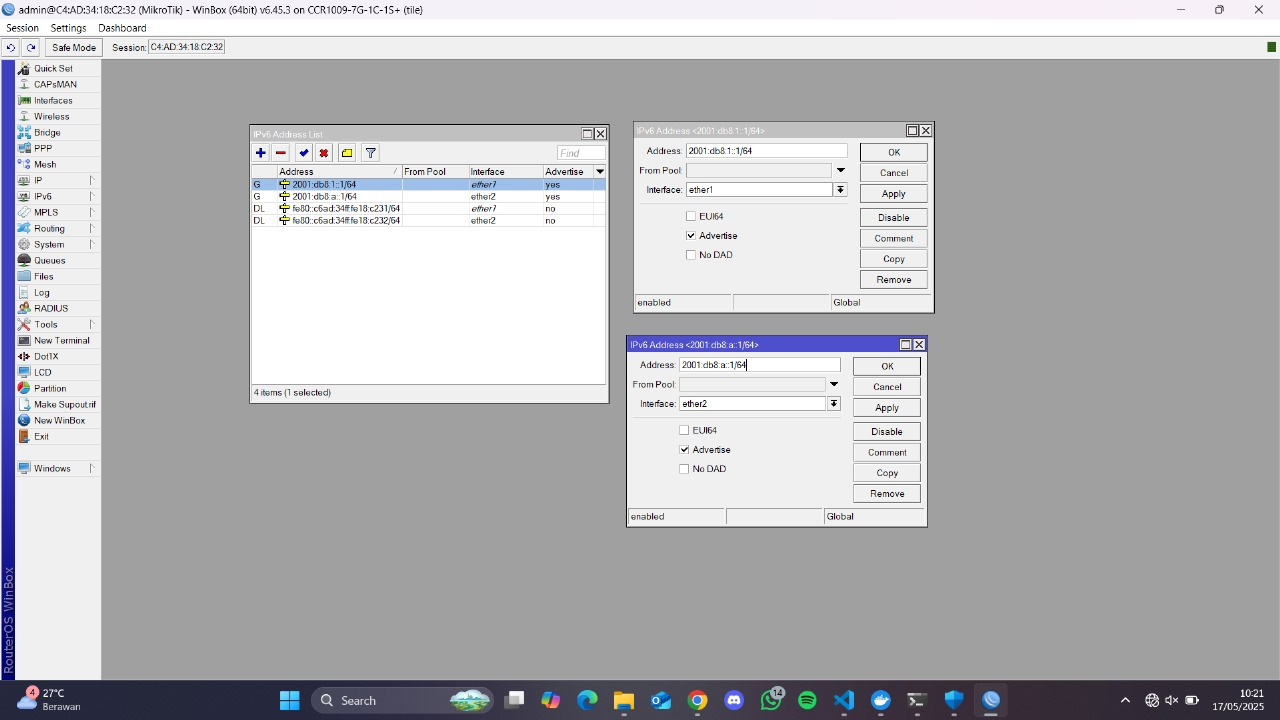
\includegraphics[width=\linewidth]{image/statis2.jpg}
      \caption{Laptop 1}
    \end{subfigure}
    \hspace{1cm}
    \begin{subfigure}[b]{0.3\linewidth}
      \centering
      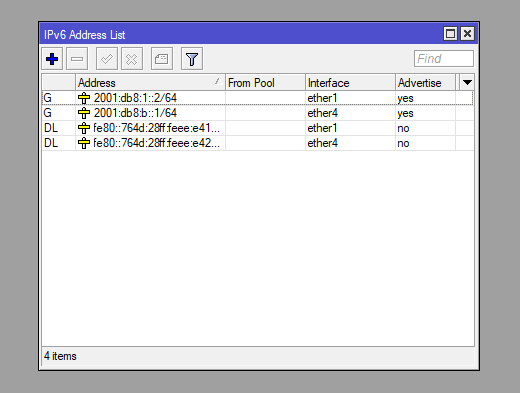
\includegraphics[width=\linewidth]{image/statis1.png}
      \caption{Laptop 2}
    \end{subfigure}
    \caption{Konfigurasi IP Address untuk ether 1 dan 2 pada masing-masing laptop}
\end{figure}
3. Konfigurasi Routing Statis (note lakukan konfigurasi ini pada router A dan b) Setelah semua interface diberi IP, langkah selanjutnya adalah menambahkan rute secara manual. Masuk ke menu IPv6 → Routes, kemudian klik "+" untuk menambahkan routing. Pada Router 1 Dst. Address: 2001:db8:b::/64 ; Gateway: 2001:db8:1::2. Pada router 2 Dst. Address: 2001:db8:a::/64 ; Gateway: 2001:db8:1::1.
\begin{figure}[H]
    \centering
    \begin{subfigure}[b]{0.3\linewidth}
      \centering
      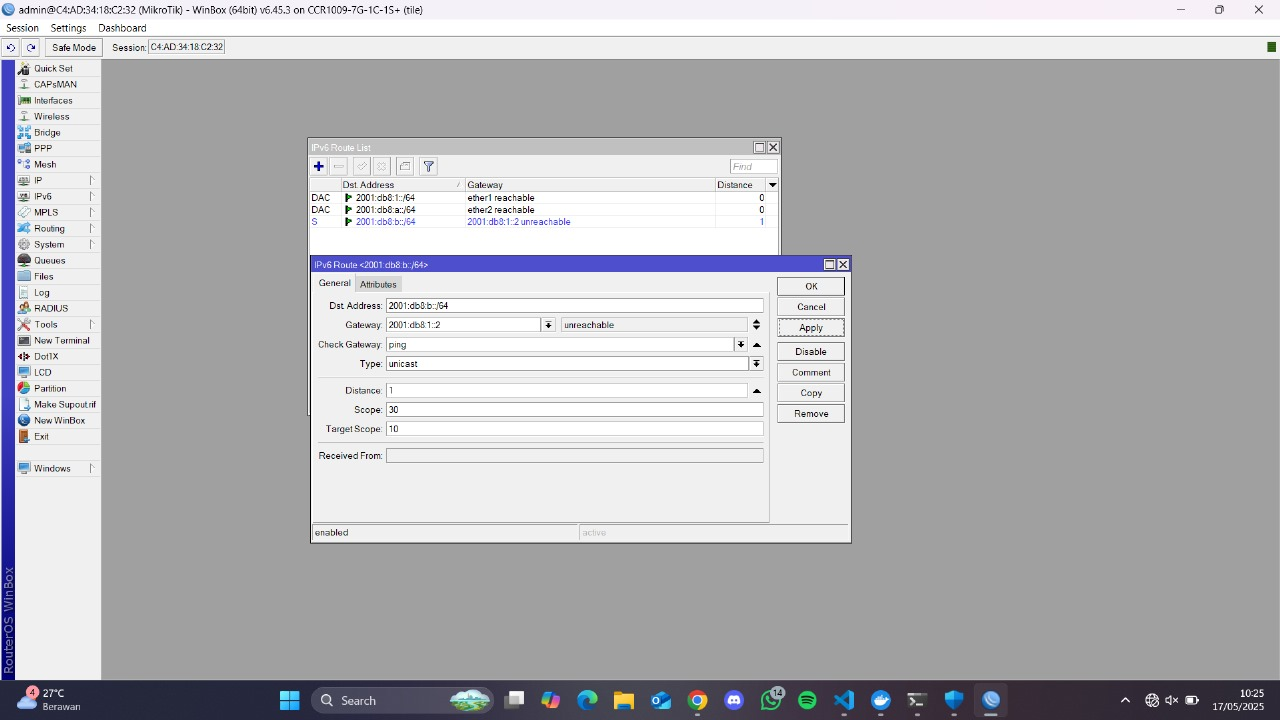
\includegraphics[width=\linewidth]{image/statis4.jpg}
      \caption{Laptop 1}
    \end{subfigure}
    \hspace{1cm}
    \begin{subfigure}[b]{0.3\linewidth}
      \centering
      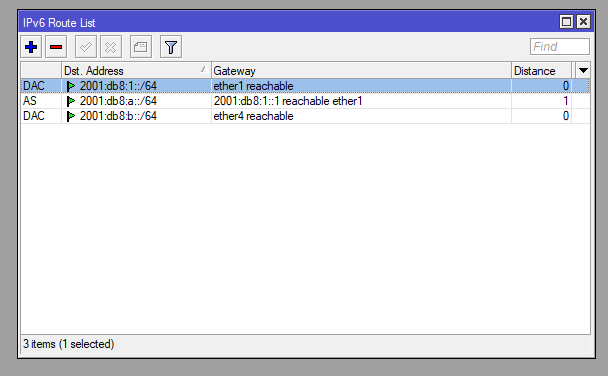
\includegraphics[width=\linewidth]{image/statis3.png}
      \caption{Laptop 2}
    \end{subfigure}
    \caption{Konfigurasi routing statis pada masing-masing laptop}
\end{figure}
4. Tes koneksi antar router dengan membuka new terminal dan uji ping pada router 1 dan 2. 
\begin{figure}[H]
    \centering
    \begin{subfigure}[b]{0.3\linewidth}
      \centering
      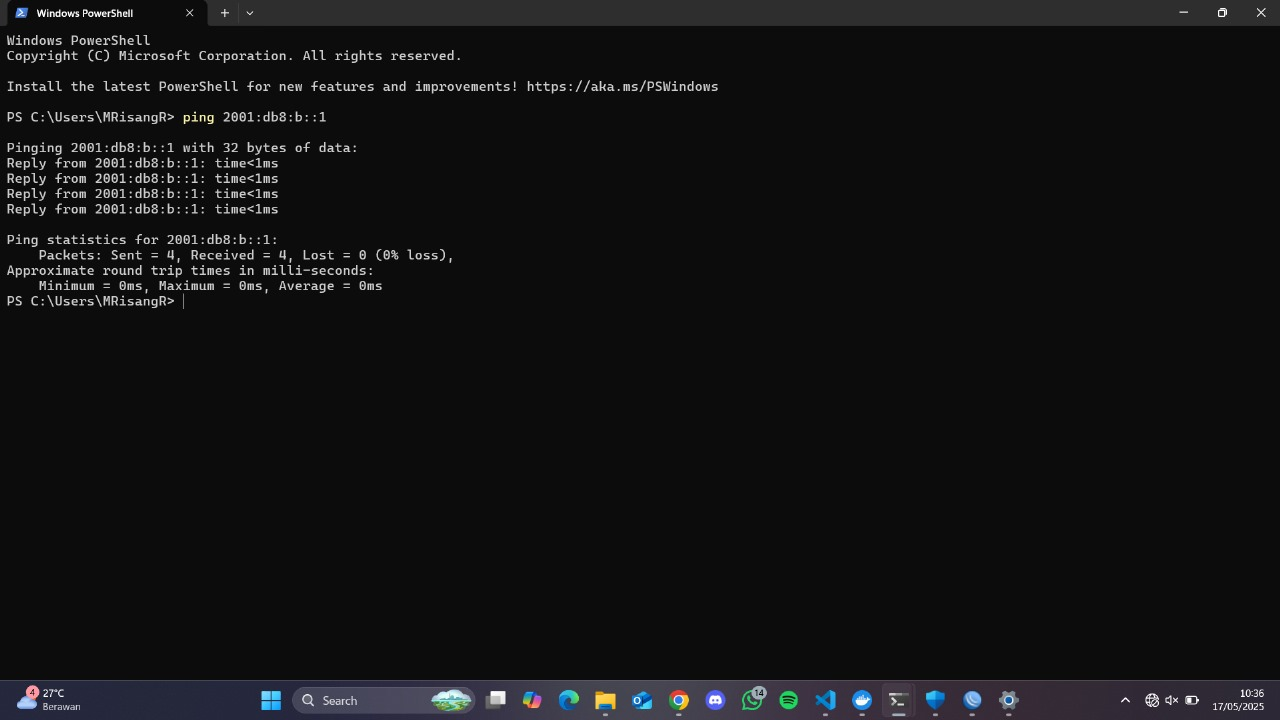
\includegraphics[width=\linewidth]{image/statis6.jpg}
      \caption{router 1 ke 2}
    \end{subfigure}
    \hspace{1cm}
    \begin{subfigure}[b]{0.3\linewidth}
      \centering
      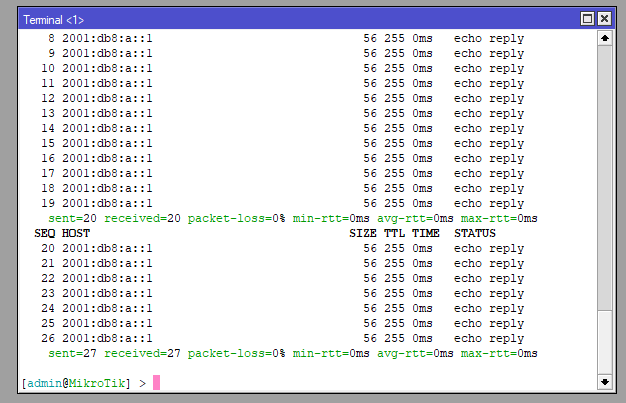
\includegraphics[width=\linewidth]{image/statis5.png}
      \caption{router 2 ke 1}
    \end{subfigure}
    \caption{Hasil ping antar router}
\end{figure}
5.Konfigurasi IP Adress di Laptop (note lakukan konfigurasi ini laptop yang terhubung pada router A dan b masing-masing) Karena ini masih menggunakan konfigurasi Static IP tambahkan IP address secara manual ke interface di laptop masing-masing bisa lewat Control Panel atau langsung di settings Windows, pastikan IP dan Gateway sudah benar sesuai Ether 2. Pada laptop yang terhubung ke Router 1, IP Address: 2001:db8:a::100 ; Prefix : /64 ; Gateway : 2001:db8:a::1 (Router1) ; DNS :2001:4860:4860::8888. Pada laptop yang terhubung ke Router 2, IP Address: 2001:db8:b::100 ; Prefix : /64 ; Gateway : 2001:db8:b::1 (Router2) ; DNS : 2001:4860:4860::8888.
\begin{figure}[H]
    \centering
    \begin{subfigure}[b]{0.3\linewidth}
      \centering
      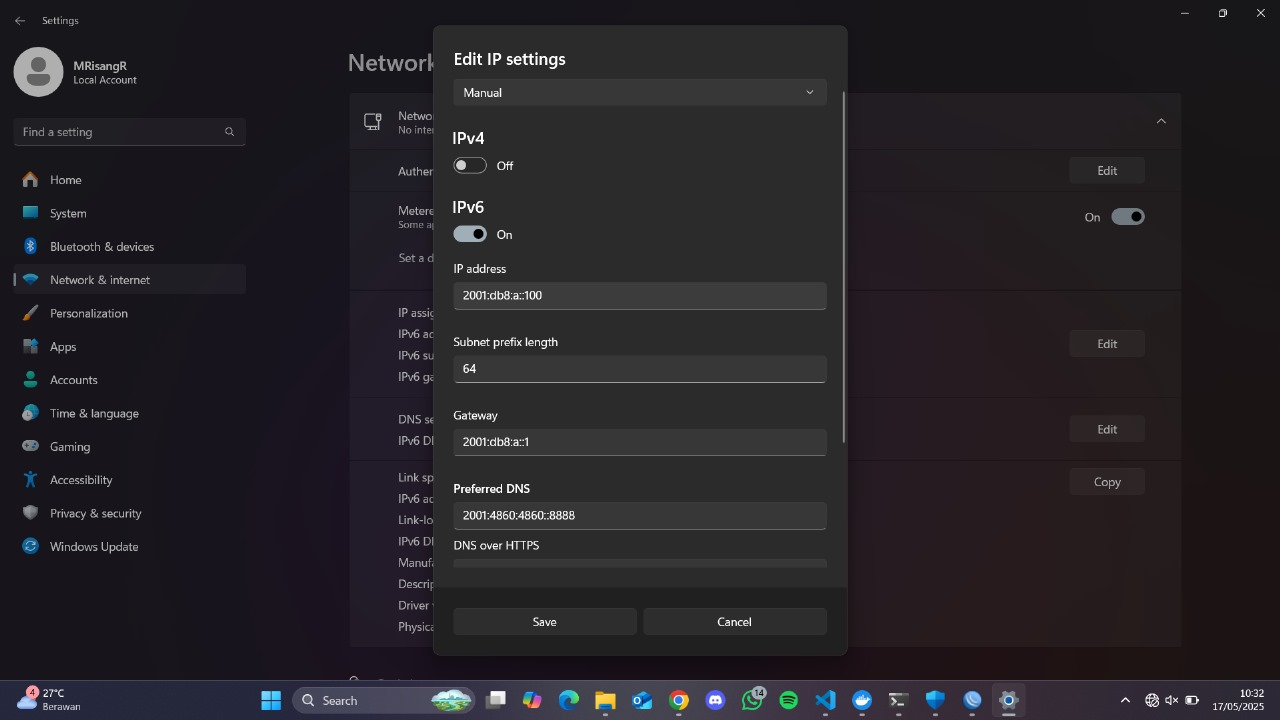
\includegraphics[width=\linewidth]{image/statis8.jpg}
      \caption{Laptop 1}
    \end{subfigure}
    \hspace{1cm}
    \begin{subfigure}[b]{0.3\linewidth}
      \centering
      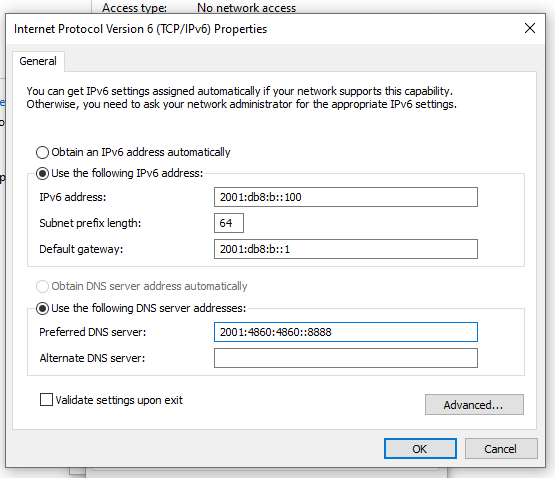
\includegraphics[width=\linewidth]{image/statis7.png}
      \caption{Laptop 2}
    \end{subfigure}
    \caption{Konfigurasi IP Address pada laptop}
\end{figure}
6. Uji test PING dari Laptop 1 ke alamat Laptop 2 dan sebaliknya. 
\begin{figure}[H]
    \centering
    \begin{subfigure}[b]{0.3\linewidth}
      \centering
      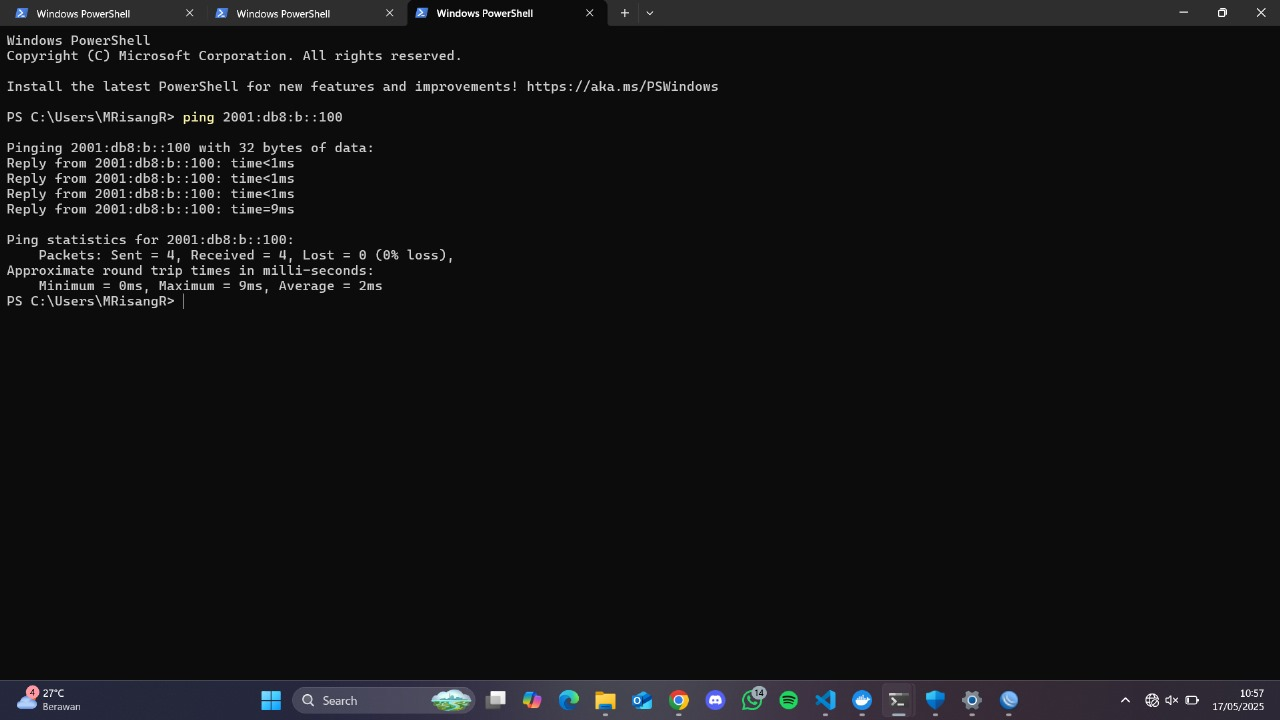
\includegraphics[width=\linewidth]{image/statis10.jpg}
      \caption{Laptop 1}
    \end{subfigure}
    \hspace{1cm}
    \begin{subfigure}[b]{0.3\linewidth}
      \centering
      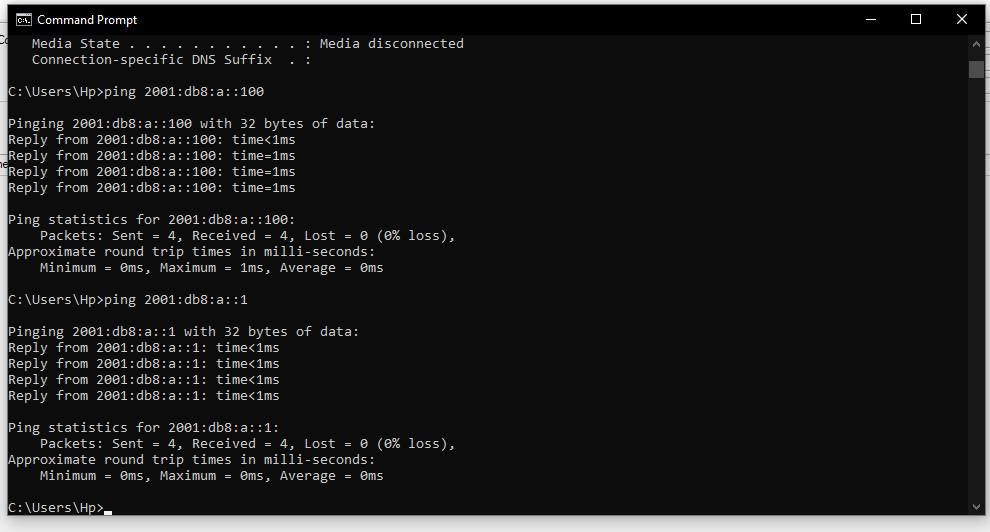
\includegraphics[width=\linewidth]{image/statis9.png}
      \caption{Laptop 2}
    \end{subfigure}
    \caption{Uji ping di cmd}
\end{figure}

\subsection{Routing Dinamis IPv6}
1. Konfigurasi IP Address pada Ether1 (note lakukan konfigurasi ini pada router A dan b) Tambahkan IP address pada ether1 yang digunakan sebagai jalur antar-router. Karena hanya ada dua perangkat yang terhubung (router A dan router B), IP ether1 Router A : 2001:db8:1::1/64 ; IP ether 1 Router B : 2001:db8:1::2/64. \\
2. Konfigurasi IP Address untuk Jaringan LAN (note lakukan konfigurasi ini pada router A dan b) Tambahkan IP address pada ether 2 yang digunakan untuk menghubungkan Laptop dengan Router. IP ether 2 Router A : 2001:db8:a::1/64 ; IP ether 2 Router B : 2001:db8:b::1/64.
\begin{figure}[H]
    \centering
    \begin{subfigure}[b]{0.3\linewidth}
      \centering
      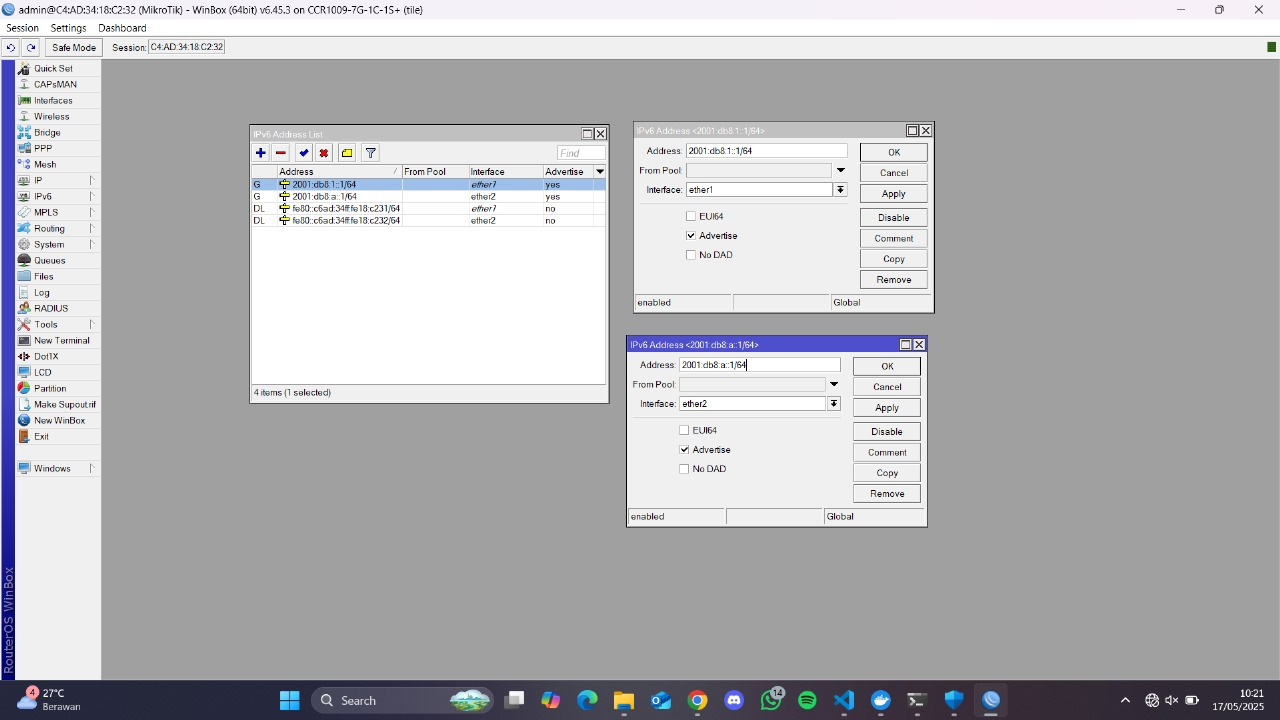
\includegraphics[width=\linewidth]{image/statis2.jpg}
      \caption{Laptop 1}
    \end{subfigure}
    \hspace{1cm}
    \begin{subfigure}[b]{0.3\linewidth}
      \centering
      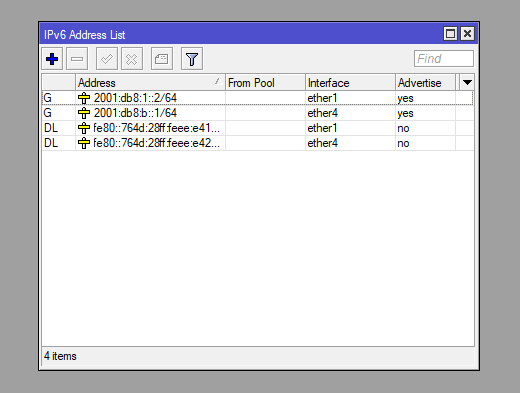
\includegraphics[width=\linewidth]{image/statis1.png}
      \caption{Laptop 2}
    \end{subfigure}
    \caption{Konfigurasi IP Address untuk ether 1 dan 2 pada masing-masing laptop}
\end{figure}
3. Konfigurasi Routing Dinamis (note lakukan konfigurasi ini pada router A dan b) Setelah semua interface diberi IP, langkah selanjutnya adalah menggunakan OSPFv3 untuk Routing Dinamis. \\
4. Buat Instance OSPFv3. Masuk ke menu IIPv6 > Routing > OSPFv3 > Instances → Klik + untuk menambahkan routing. Name: ospf-instance. Router ID: misalnya 1.1.1.1 untuk Router1, 2.2.2.2 untuk Router2.
\begin{figure}[H]
    \centering
    \begin{subfigure}[b]{0.3\linewidth}
      \centering
      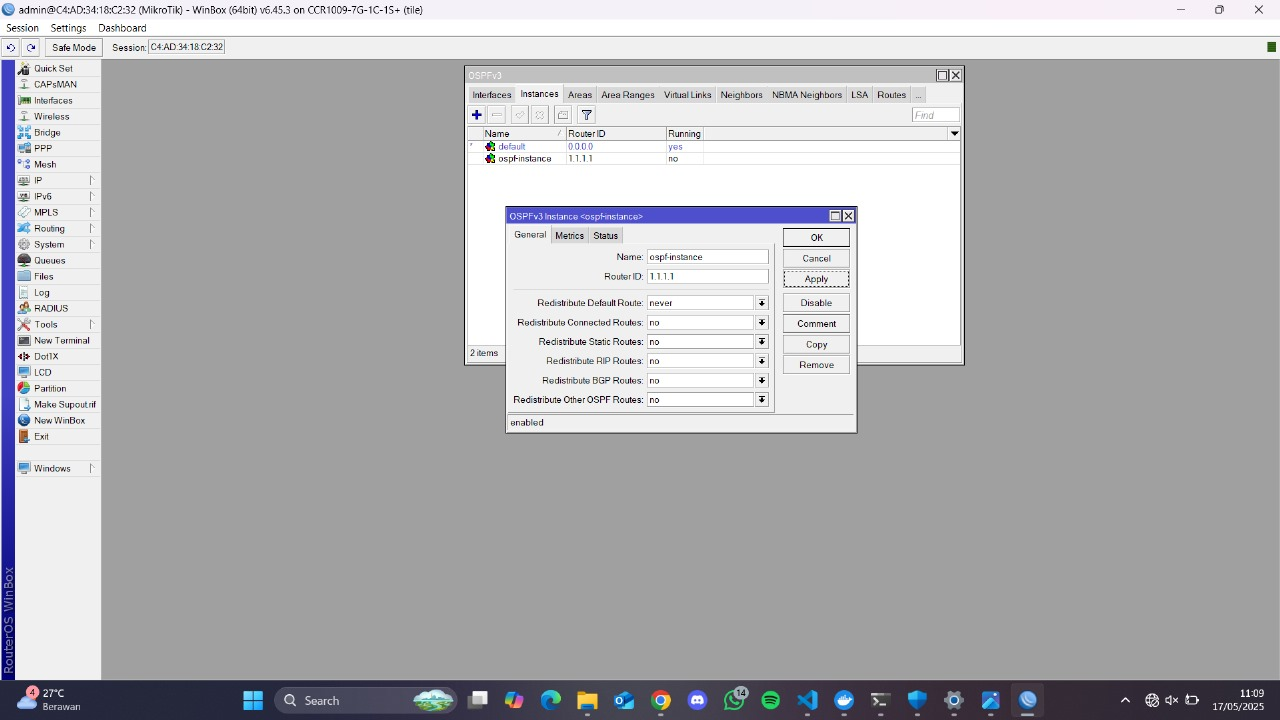
\includegraphics[width=\linewidth]{image/dinamis2.jpg}
      \caption{router 1}
    \end{subfigure}
    \hspace{1cm}
    \begin{subfigure}[b]{0.3\linewidth}
      \centering
      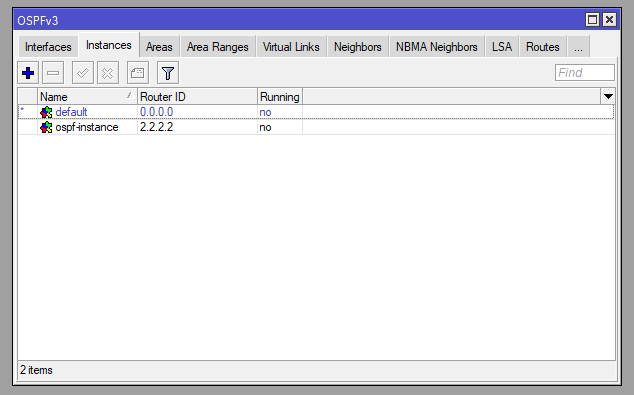
\includegraphics[width=\linewidth]{image/dinamis1.png}
      \caption{router 2}
    \end{subfigure}
    \caption{Instance OSPFv3}
\end{figure}
5. Tambah Area. Masuk ke menu Routing > OSPFv3 > Areas → Klik +. Name: backbone ; Instance: pilih ospf-instance ; Area ID: 0.0.0.0 (wajib untuk backbone area).
\begin{figure}[H]
    \centering
    \begin{subfigure}[b]{0.3\linewidth}
      \centering
      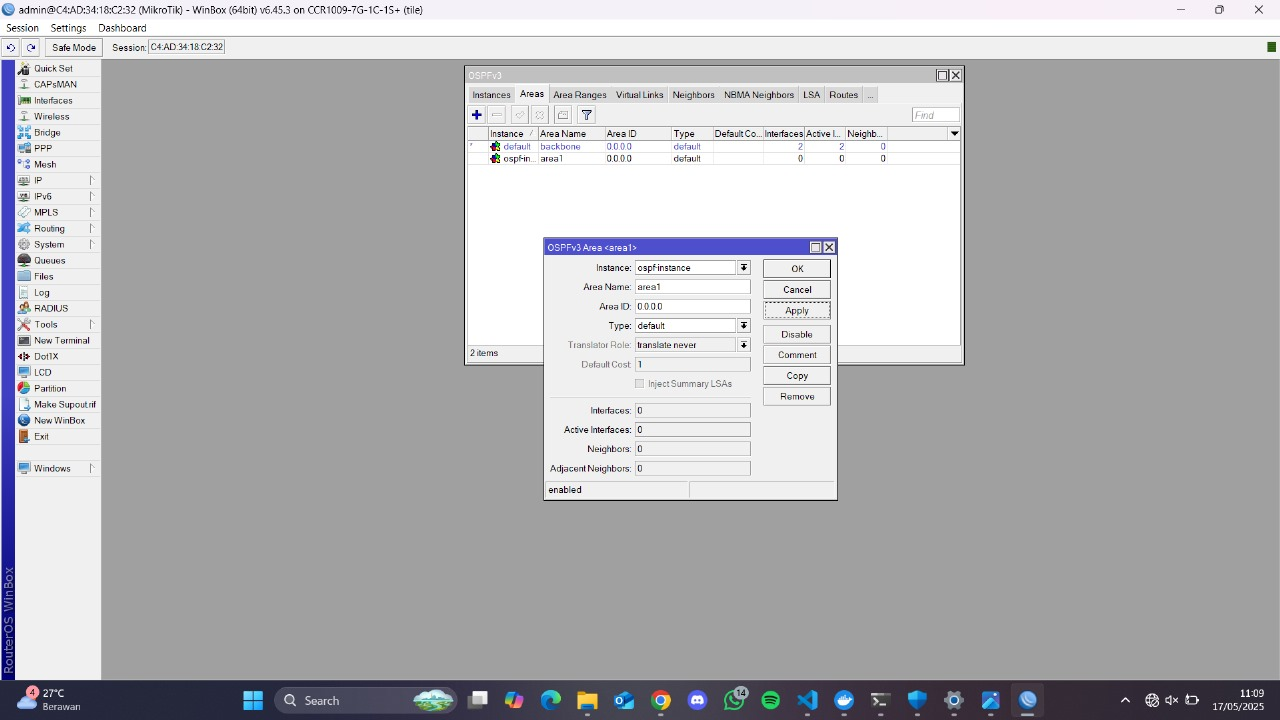
\includegraphics[width=\linewidth]{image/dinamis4.jpg}
      \caption{Laptop 1}
    \end{subfigure}
    \hspace{1cm}
    \begin{subfigure}[b]{0.3\linewidth}
      \centering
      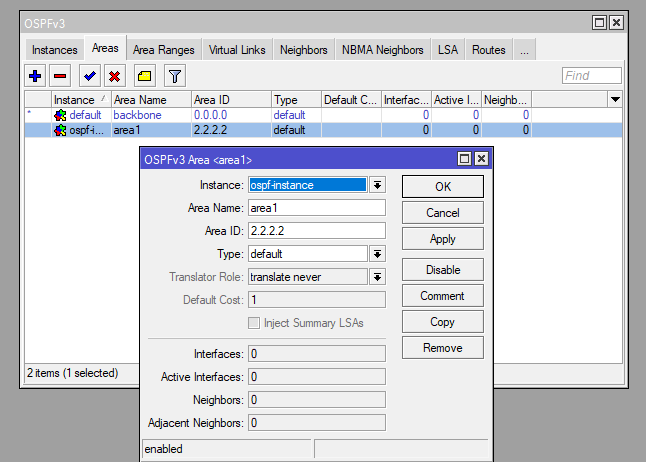
\includegraphics[width=\linewidth]{image/dinamis3.png}
      \caption{Laptop 2}
    \end{subfigure}
    \caption{Area OSPFv3}
\end{figure}
6. Tambah Interface OSPFv3. Router1: Masuk ke menu Routing > OSPFv3 > Interface → Klik + ; Interface: ether1 (ke Router2) ; Instance: ospf-instance ; Area: backbone Tambahkan juga interface LAN: Interface: ether2. Router2: Tambahkan interface ether1 dan ether2 dengan cara yang sama.
\begin{figure}[H]
    \centering
    \begin{subfigure}[b]{0.3\linewidth}
      \centering
      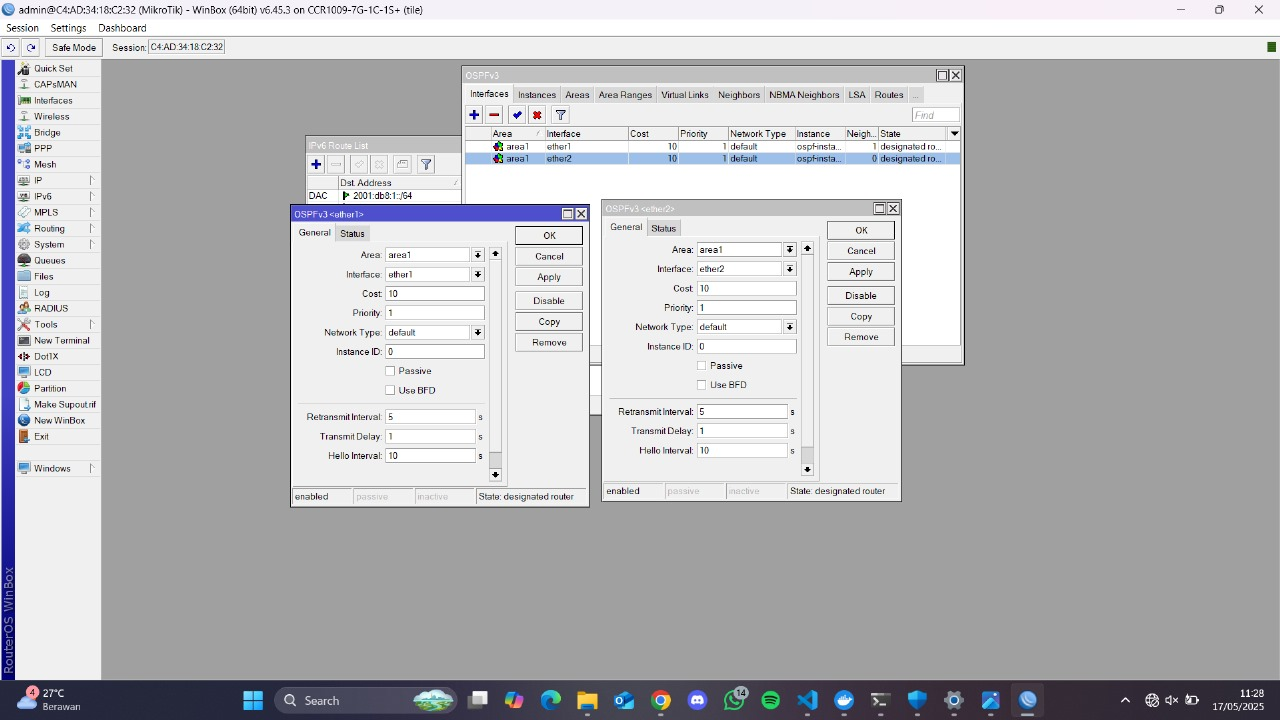
\includegraphics[width=\linewidth]{image/dinamis6.jpg}
      \caption{router 1}
    \end{subfigure}
    \hspace{1cm}
    \begin{subfigure}[b]{0.3\linewidth}
      \centering
      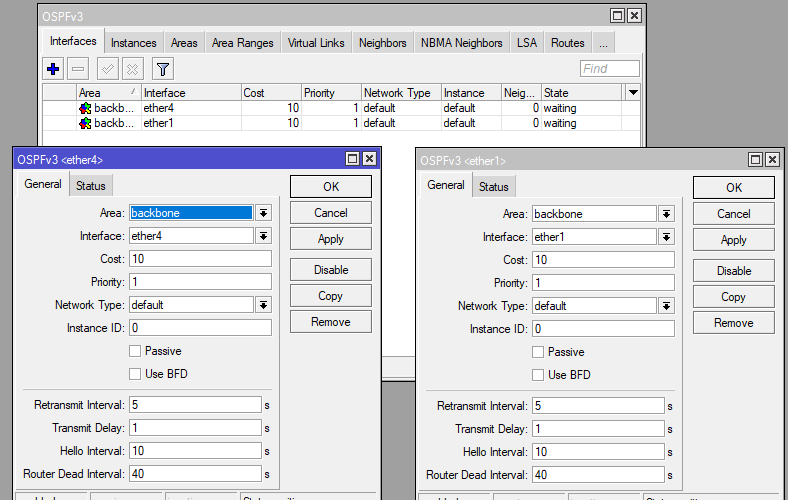
\includegraphics[width=\linewidth]{image/dinamis5.png}
      \caption{router 2}
    \end{subfigure}
    \caption{Interface OSPFv3}
\end{figure}
7. Cek Neighbor dan Routing Masuk ke menu Routing > OSPFv3 > Neighbors. Harus muncul tetangga OSPF antara Router1 dan Router2 Optional coba cek Masuk ke menu IPv6 > Routes. Harus terlihat rute dinamis ke jaringan 2001:db8:a::/64 dan 2001:db8:b::/64.
\begin{figure}[H]
    \centering
    \begin{subfigure}[b]{0.3\linewidth}
      \centering
      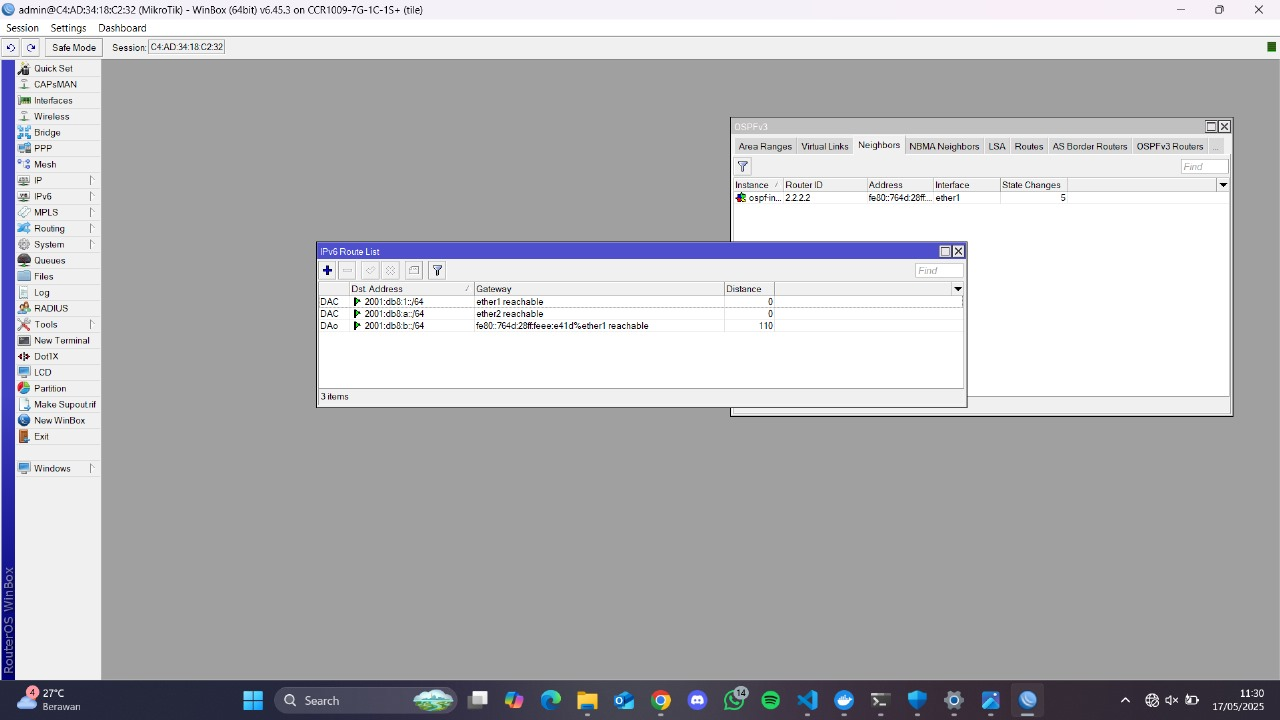
\includegraphics[width=\linewidth]{image/dinamis8.jpg}
      \caption{router 2 terlihat router 1}
    \end{subfigure}
    \hspace{1cm}
    \begin{subfigure}[b]{0.3\linewidth}
      \centering
      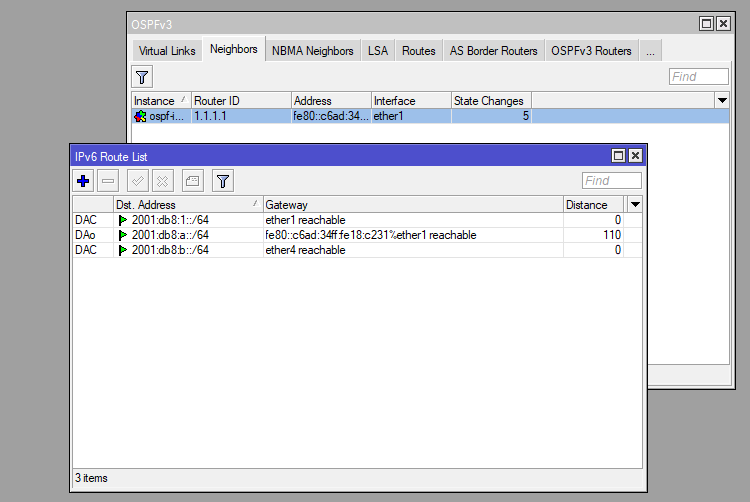
\includegraphics[width=\linewidth]{image/dinamis7.png}
      \caption{router 1 terlihat pada router 2}
    \end{subfigure}
    \caption{Neighbor dan route list antar tetangga router}
\end{figure}
8. Konfigurasi IP Adress di Laptop (note lakukan konfigurasi ini laptop yang terhubung pada router A dan b masing-masing) Karena ini masih menggunakan konfigurasi Static IP tambahkan IP address secara manual ke interface di laptop masing-masing bisa lewat Control Panel atau langsung di settings Windows, pastikan IP dan Gateway sudah benar sesuai Ether 2. Pada laptop yang terhubung ke Router 1, IP Address: 2001:db8:a::100 ; Prefix : /64 ; Gateway : 2001:db8:a::1 (Router1) ; DNS : 2001:4860:4860::8888. Pada laptop yang terhubung ke Router 2, IP Address: 2001:db8:b::100 ; Prefix : /64 ; Gateway : 2001:db8:b::1 (Router2) ; DNS : 2001:4860:4860::8888.
\begin{figure}[H]
    \centering
    \begin{subfigure}[b]{0.3\linewidth}
      \centering
      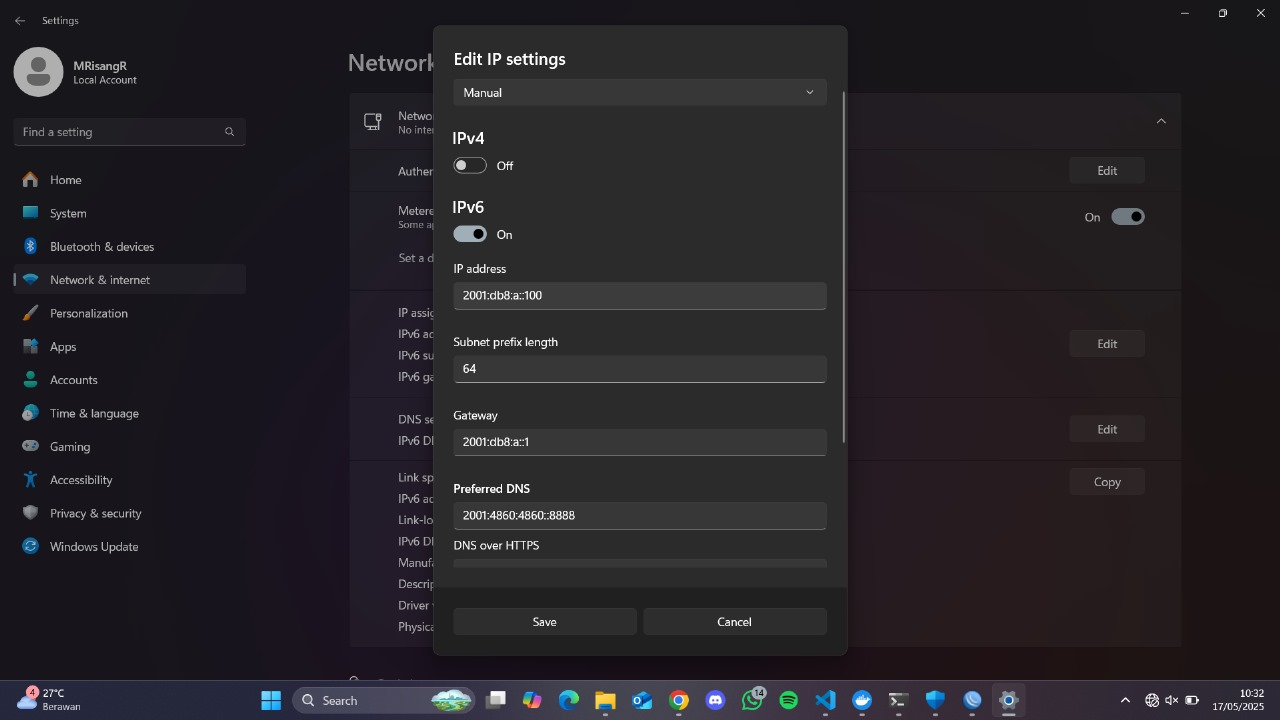
\includegraphics[width=\linewidth]{image/statis8.jpg}
      \caption{Laptop 1}
    \end{subfigure}
    \hspace{1cm}
    \begin{subfigure}[b]{0.3\linewidth}
      \centering
      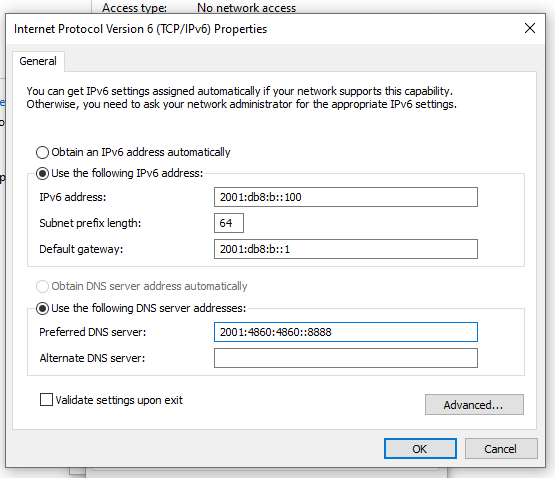
\includegraphics[width=\linewidth]{image/statis7.png}
      \caption{Laptop 2}
    \end{subfigure}
    \caption{Konfigurasi IP Address pada laptop}
\end{figure}
9.  Uji test PING dari Laptop 1 ke alamat Laptop 2 dan sebaliknya. 
\begin{figure}[H]
    \centering
    \begin{subfigure}[b]{0.3\linewidth}
      \centering
      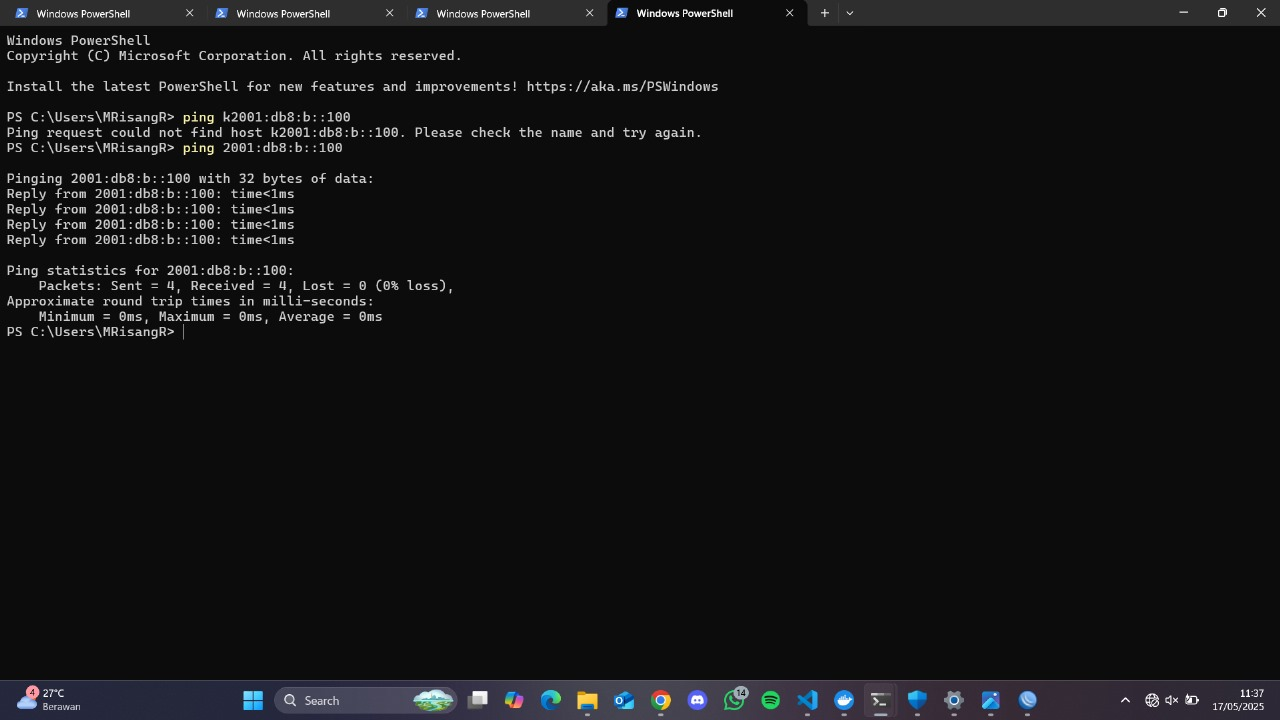
\includegraphics[width=\linewidth]{image/dinamis10.jpg}
      \caption{Laptop 1}
    \end{subfigure}
    \hspace{1cm}
    \begin{subfigure}[b]{0.3\linewidth}
      \centering
      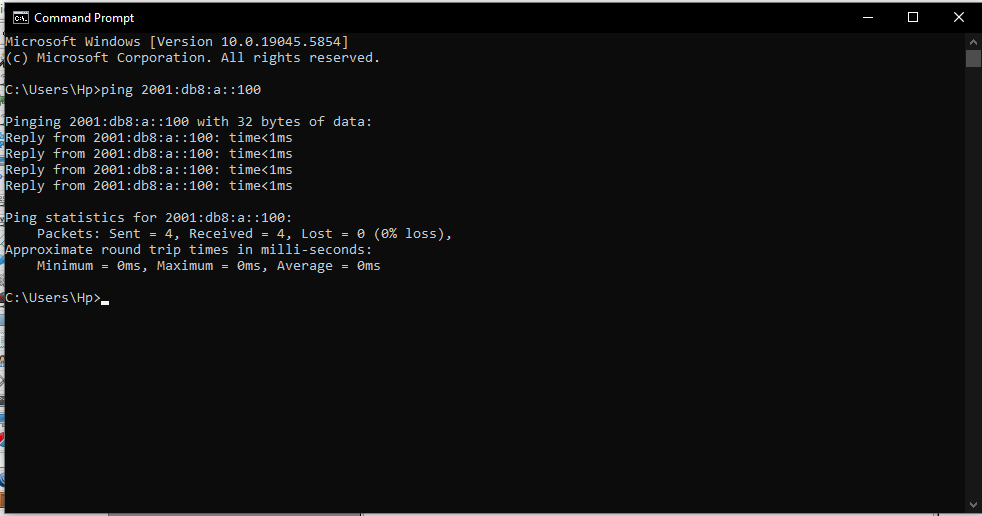
\includegraphics[width=\linewidth]{image/dinamis9.png}
      \caption{Laptop 2}
    \end{subfigure}
    \caption{Uji ping di cmd}
\end{figure}

\section{Analisis Hasil Percobaan}
Pada praktikum Modul 2, praktikan melakukan kegiatan berupa routing IPv6 statis dan dinamis. Tujuan praktikum modul 2 ini adalah memahami implementasi pengalamatan IPv6, proses subnetting, serta konfigurasi routing statis dan dinamis menggunakan perangkat jaringan (Mikrotik) atau simulator jaringan seperti GNS3.
\subsection{Perbandingan Hasil Percobaan dengan Teori}
Berdasarkan teori, pada implementasi Subnetting IPv6 memungkinkan pembagian alamat sangat besar. Dari satu blok /32, bisa dibuat 65.536 subnet /48, dan dari /48 ke /64 bisa dibuat 65.536 subnet lagi. Hasil yang diperoleh Praktikan berhasil membagi 2001:db8::/32 menjadi empat subnet /64 untuk empat antarmuka router. \\ 
Pada konfigurasi IP Address dan routing statis, berdasarkan teori Routing statis digunakan untuk jaringan kecil dan tidak berubah-ubah. Rute diatur manual. Hasil yang diperoleh Semua konfigurasi ditampilkan lengkap dengan contoh IP yang valid (2001:db8:a::1, dll). Ping antar laptop berhasil, artinya routing statis bekerja. \\
Pada konfigurasi routing dinamis, berdasarkan teori OSPFv3 adalah protokol routing dinamis untuk IPv6. Digunakan dalam jaringan besar agar rute dapat berubah otomatis sesuai topologi. Hasil yang diperoleh koneksi antar router dan ping ke LAN router lain berfungsi. Neighbor OSPF terbentuk.
\subsection{Faktor yang Mempengaruhi Hasil}
Pada saat proses routing dinamis, terdapat kerusakan pada kabel LAN yang membuat waktu praktikum sedikit terhambat. \\
Pada saat menambahkan area pada OSPFv3, terjadi error dengan reason tidak dapat diduplikasi sehingga saat praktikum, kami mengubah nama area yang seharusnya backbone menjadi area1 agar terbaca interface dan Neighbors.

\section{Hasil Tugas Modul}
Berikut merupakan topologi IPv6 untuk statis dan dinamis.
\begin{figure}[H]
    \centering
    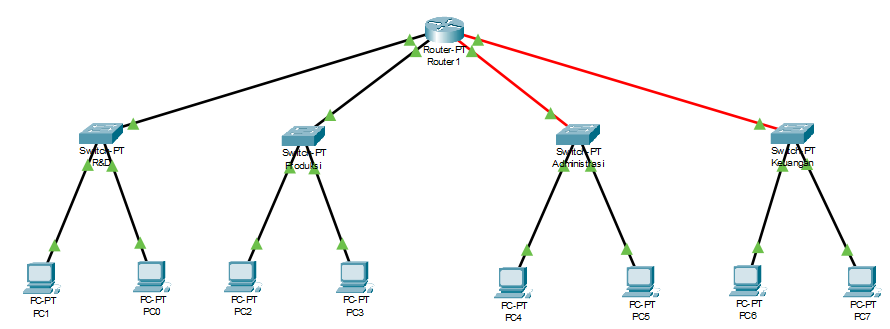
\includegraphics[width=0.5\linewidth]{image/topologi.png}
    \label{fig:inirujukan}
\end{figure}
\subsection{Statis}
\begin{figure}[H]
    \centering
    \begin{subfigure}[b]{0.3\linewidth}
      \centering
      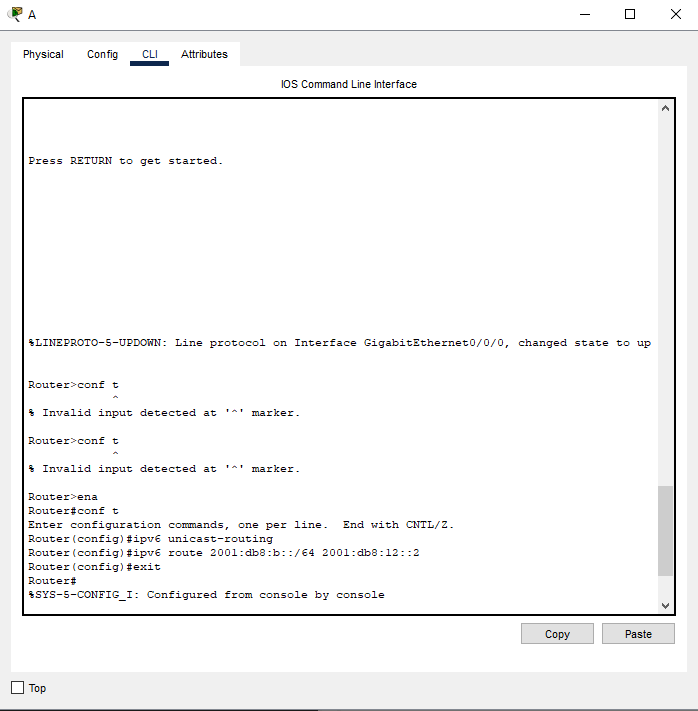
\includegraphics[width=\linewidth]{image/statiss.png}
      \caption{router A}
    \end{subfigure}
    \hspace{1cm}
    \begin{subfigure}[b]{0.3\linewidth}
      \centering
      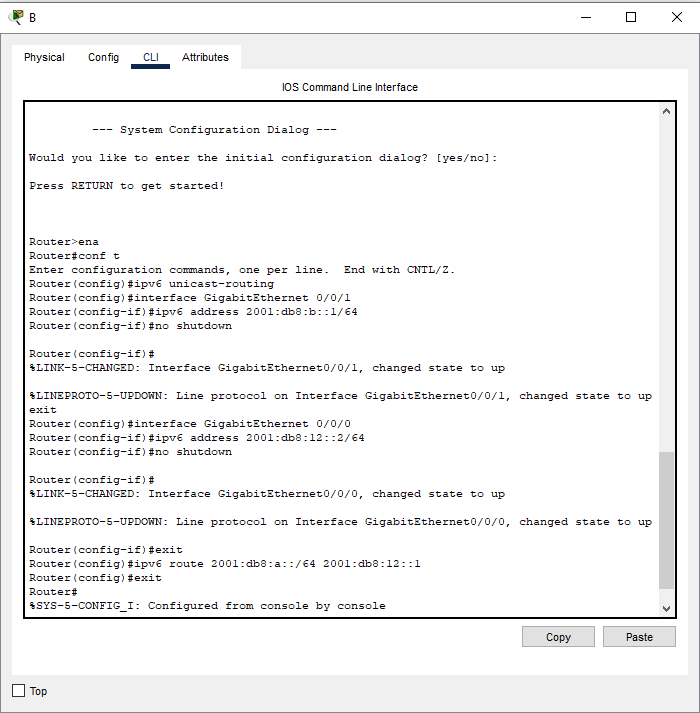
\includegraphics[width=\linewidth]{image/statisd.png}
      \caption{router B}
    \end{subfigure}
    \caption{Konfigurasi IPv6}
\end{figure}
untuk hasil ping dari PC hanya bisa ke router masing-masing tidak dapat terhubung ke PC lawan. 
\subsection{dinamis}
\begin{figure}[H]
    \centering
    \begin{subfigure}[b]{0.3\linewidth}
      \centering
      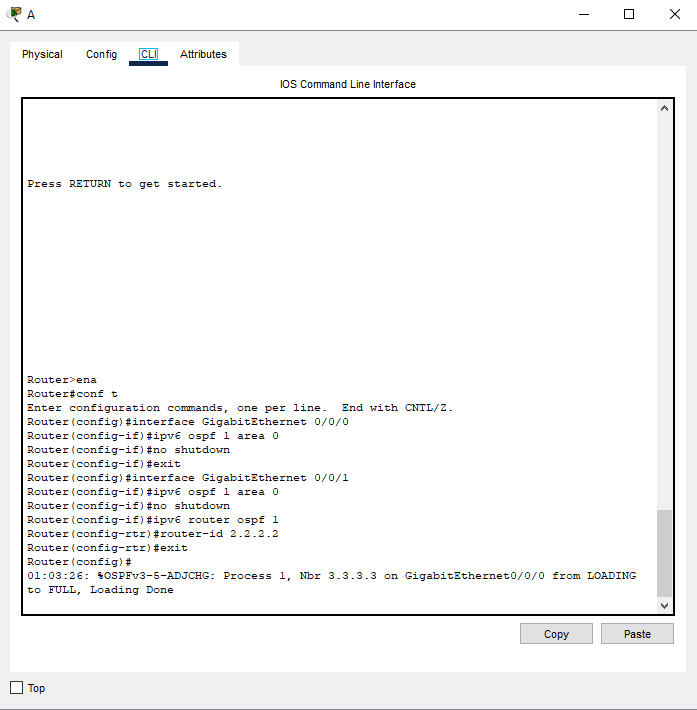
\includegraphics[width=\linewidth]{image/ospf1.png}
      \caption{router A}
    \end{subfigure}
    \hspace{1cm}
    \begin{subfigure}[b]{0.3\linewidth}
      \centering
      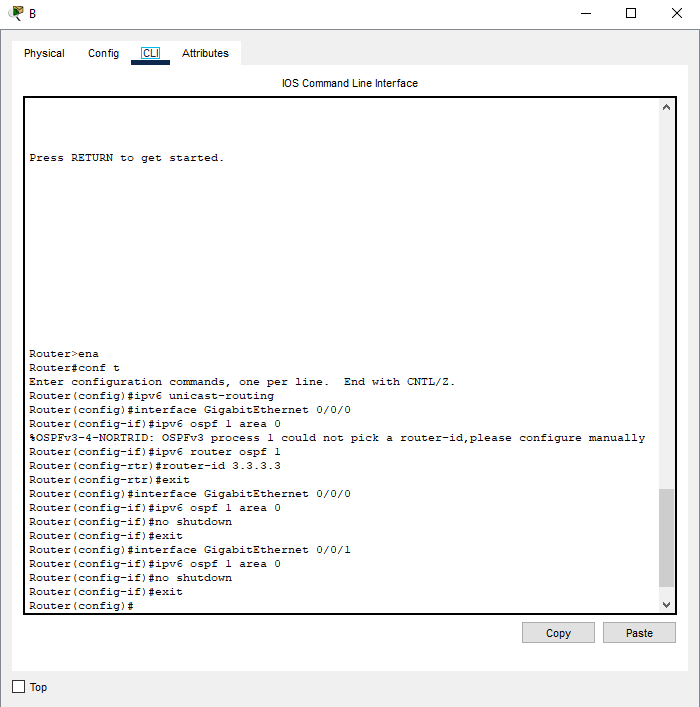
\includegraphics[width=\linewidth]{image/ospf2.png}
      \caption{router B}
    \end{subfigure}
    \caption{Penambahan ospf dan area pada router}
\end{figure}
\begin{figure}[H]
    \centering
    \begin{subfigure}[b]{0.3\linewidth}
      \centering
      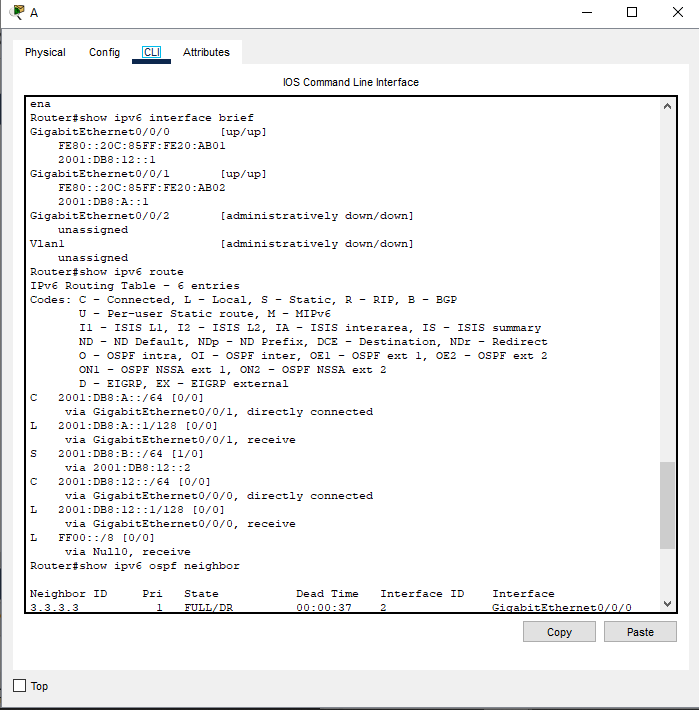
\includegraphics[width=\linewidth]{image/cekA.png}
      \caption{router A}
    \end{subfigure}
    \hspace{1cm}
    \begin{subfigure}[b]{0.3\linewidth}
      \centering
      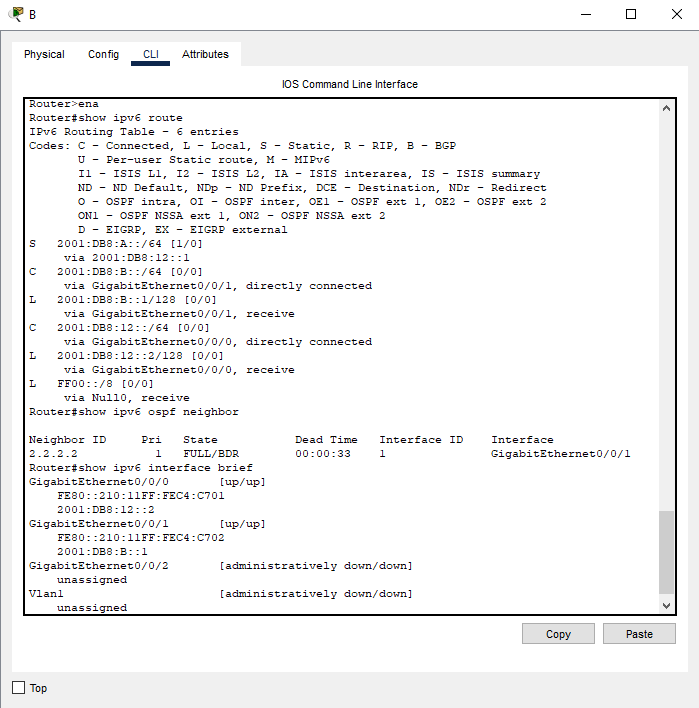
\includegraphics[width=\linewidth]{image/cekB.png}
      \caption{router B}
    \end{subfigure}
    \caption{verifikasi route dinamis dan neighbor ospf}
\end{figure}
untuk hasil ping dari PC hanya bisa ke router masing-masing dan tidak dapat terhubung ke PC lawan.
\begin{figure}[H]
    \centering
    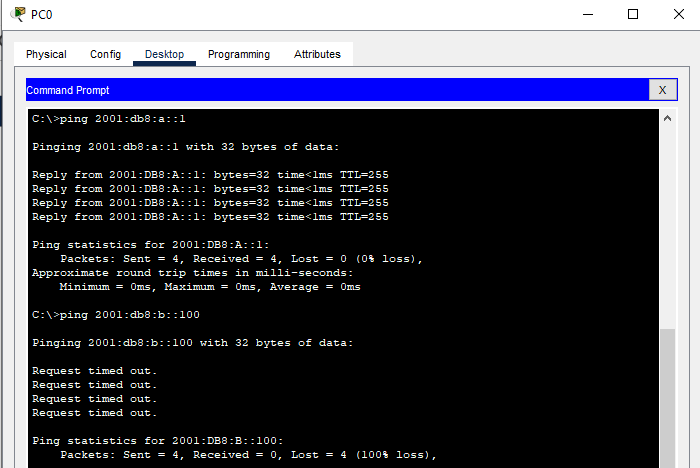
\includegraphics[width=0.5\linewidth]{image/hasil.png}
    \label{fig:inirujukan}
\end{figure}

\section{Kesimpulan}
Praktikum pada Modul 2 bertujuan untuk memberikan pemahaman dan keterampilan teknis dalam mengimplementasikan pengalamatan IPv6 serta manajemen routing menggunakan metode statis dan dinamis di jaringan berbasis Mikrotik. Seluruh rangkaian kegiatan praktikum telah berhasil dilaksanakan, mulai dari pengalokasian subnet IPv6, konfigurasi IP pada antarmuka router dan laptop, hingga pengujian konektivitas menggunakan ping antar perangkat. Secara keseluruhan, hasil yang diperoleh sesuai dengan teori. Praktikan mampu melakukan proses subnetting dari blok 2001:db8::/32 menjadi beberapa subnet /64 dengan benar. Konfigurasi routing statis menunjukkan bahwa komunikasi antar jaringan berjalan lancar ketika tabel rute diatur secara manual. Begitu pula pada implementasi routing dinamis menggunakan OSPFv3, rute dapat terbentuk secara otomatis dan konektivitas tetap terjaga, membuktikan bahwa protokol dinamis bekerja dengan baik sebagaimana yang dijelaskan dalam teori. Melalui praktikum ini, praktikan memperoleh pemahaman mendalam mengenai struktur dan keunggulan IPv6, termasuk mekanisme auto-configuration, ruang alamat yang luas, serta penerapan protokol routing.

\section{Lampiran}
\subsection{Dokumentasi saat praktikum}
\begin{figure}[H]
    \centering
    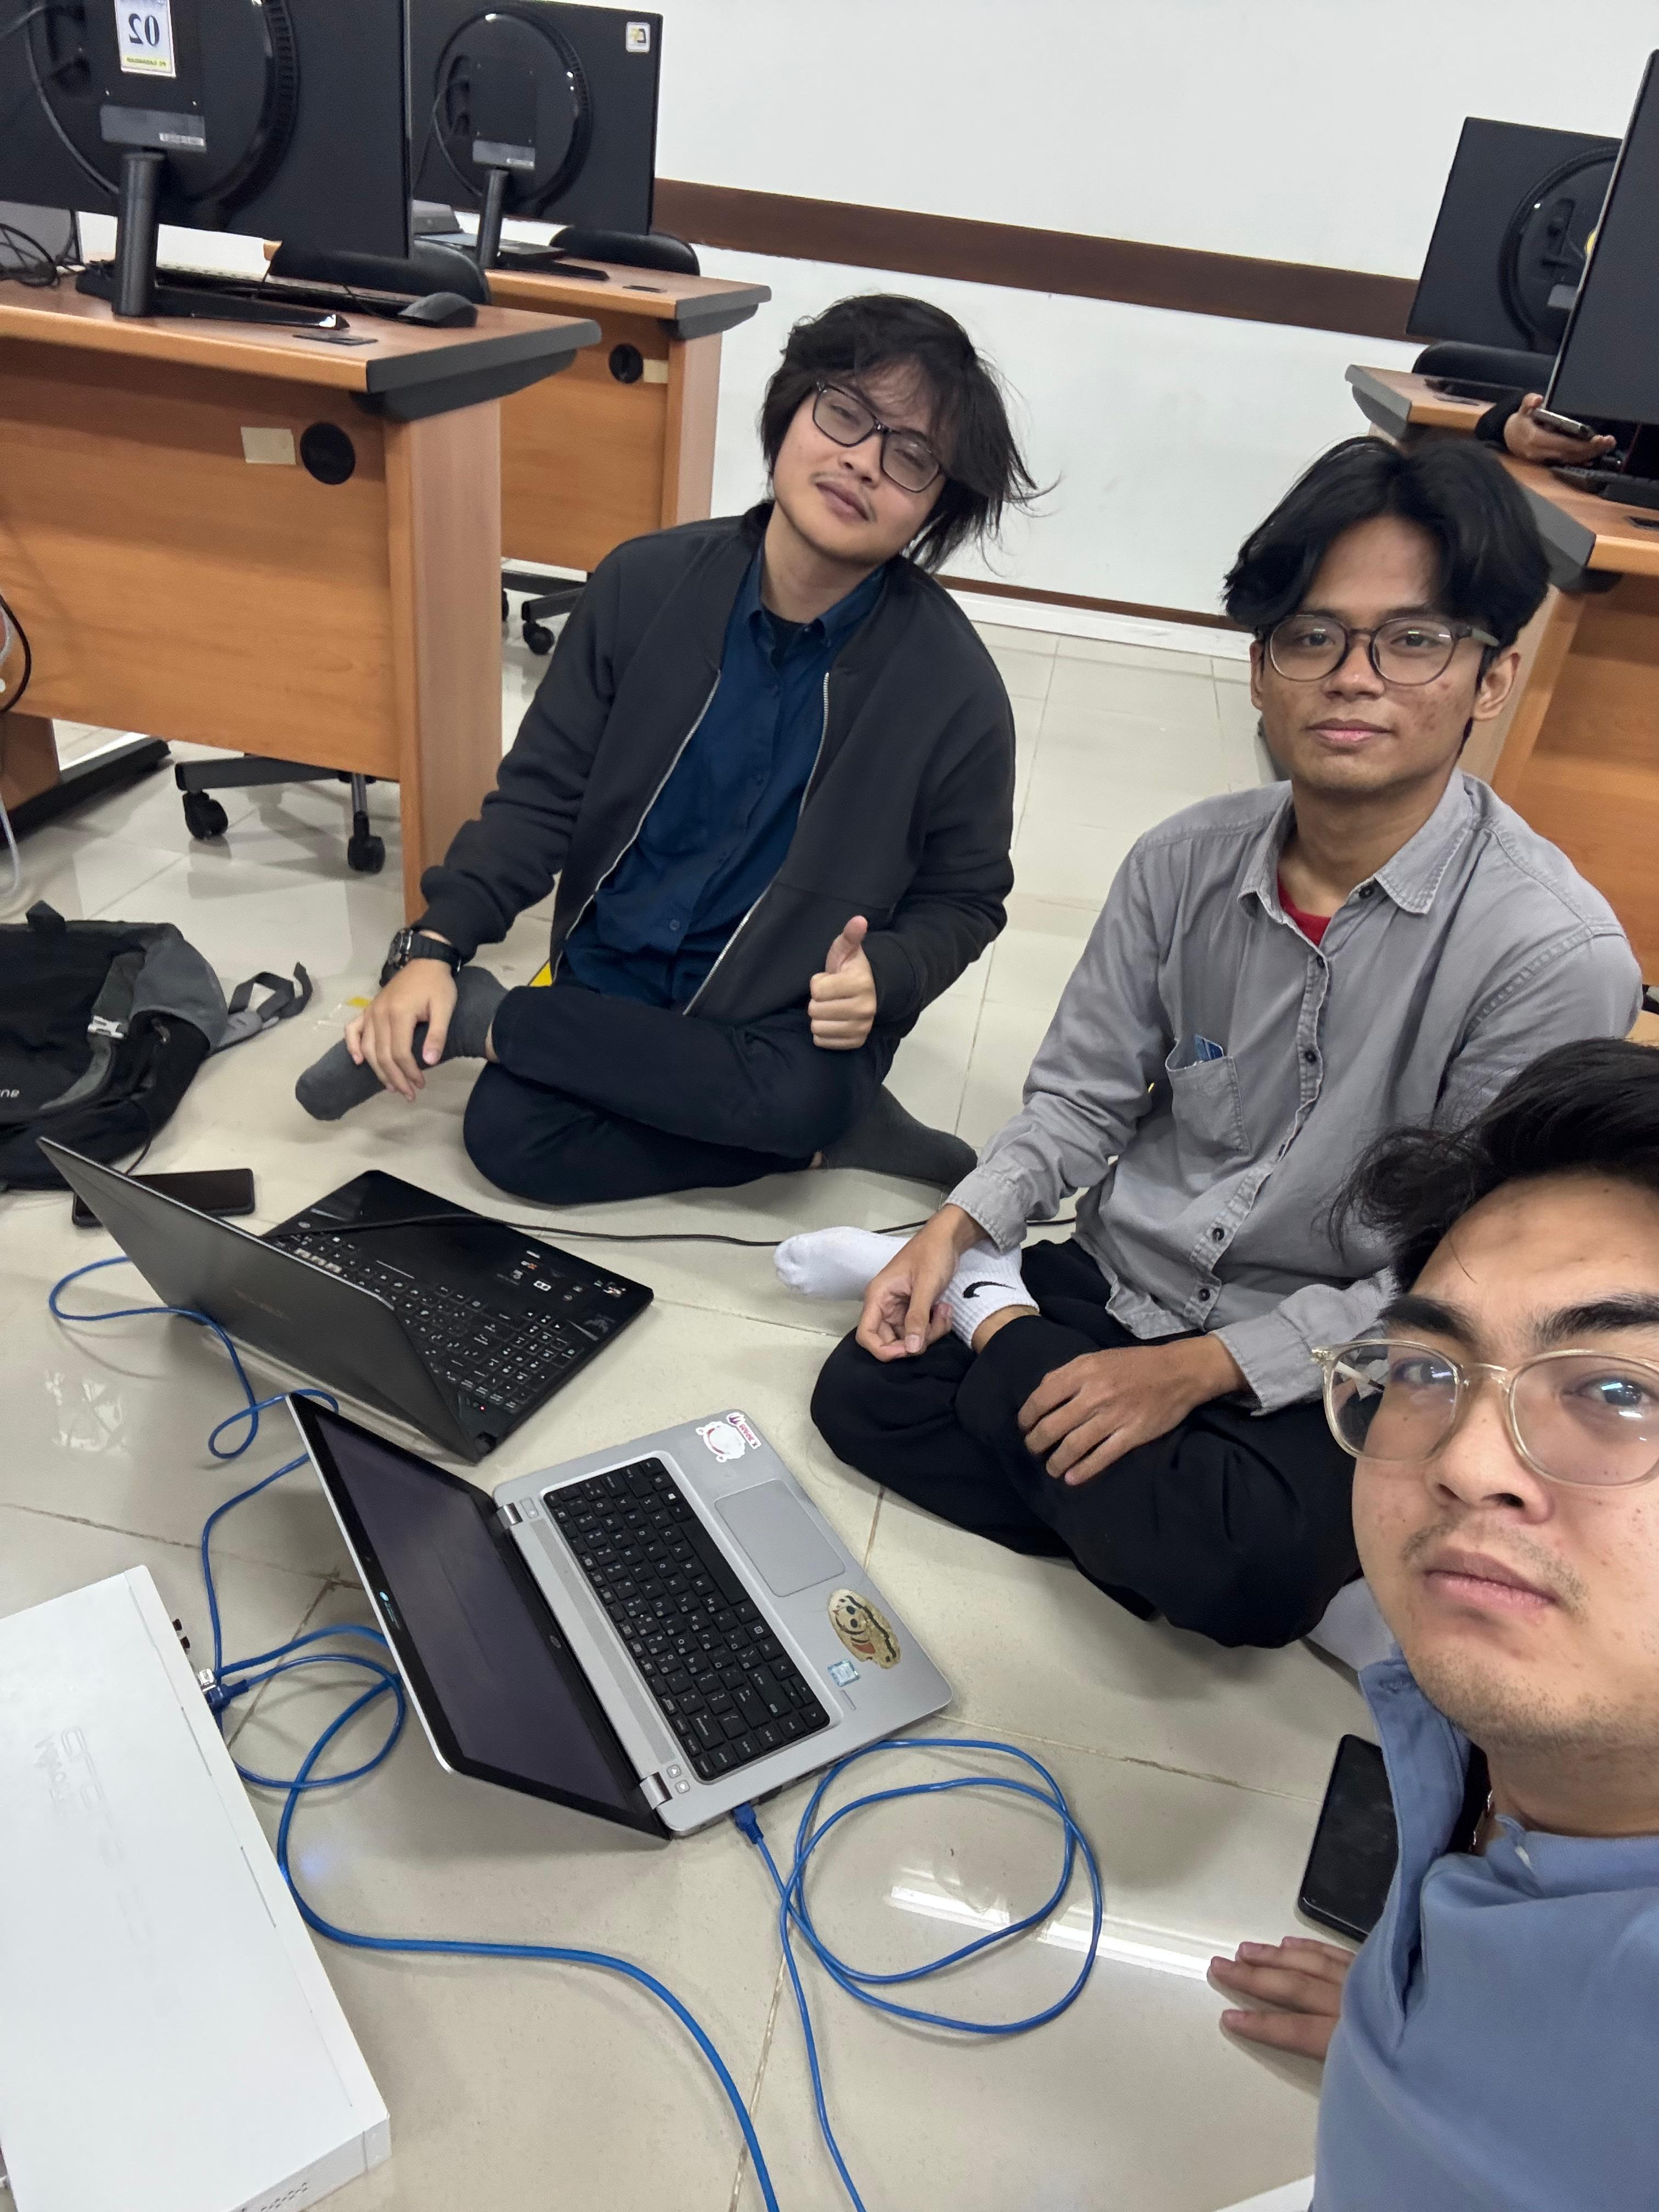
\includegraphics[width=0.65\linewidth]{image/lampiran.jpg}
    \label{fig:inirujukan}
\end{figure}



\end{document}